\section{Formal verification in presence of unbounded loops\label{sec-motor-control}}

Many programs targeting REDFIN share the distinctive feature of
the energy estimation program considered in section~\ref{sec-verification},
i.e. the existence of an  upper \emph{bound on execution time},
thanks to the fact that their termination does not
depend on the input data. However, other programs may have loops
which are guarded by termination conditions that involve computation
considering the input parameters of the program, thus making the loop
\emph{unbounded}.

Presence of unbounded loops makes program verification by symbolic execution considerably
harder~\cite[p.~50:20]{SurveySymExec-CSUR18}, since the number of program execution
paths becomes infinite. In this section we apply the developed verification framework
to a larger example of a stepper motor control program and verify one of its essential
safety properties by formulating it as a~\emph{loop invariant} and ensuring that the
invariant holds for every possible state of the loop.

\subsection{Stepper motor control program}

Stepper motors are often deployed as parts of antenna and solar panel pointing units
in space satellites. We consider a program for controlling a motor with
one degree of freedom. The program, given the distance to move the motor and safety
bounds on velocity and acceleration, will

The algorithm~\ref{alg-motor} expects three input
parameters: $dist$ --- the distance to move the motor, $v\_max$ --- the maximal permitted
velocity and $a\_max$ --- the maximal permitted acceleration and computes a series of
speed and velocity values that will be used to move the motor. The conditional statement on
starting in line 9 decides whether to accelerate the motor, to keep it on steady speed or
to decelerate the motor; see~\ref{fig-motor} for example plots of velocity and distance travelled
against time. The spike on the bottom-left of the velocity graph illustrates
the edge covered by the conditional statement on line 18: if the velocity is zero, but the target
distance has not yet been reached, the motor must be moved a bit further.

\begin{algorithm}[h]
  \begin{algorithmic}[1]
\Require {$dist$, $v\_max$, $a\_max$}
\State $s \gets 0$
\State $v \gets 0$
\While {$true$}
  % Compute deceleration distance based on current speed
  \State $decel\_steps\gets \lfloor v / a\_max \rfloor$
  \algorithmiccomment{Compute deceleration distance based on current speed}
  \State $s\_decel \gets a\_max \cdot (decel\_steps + 1) / 2$
  \If {$decel\_steps \cdot a\_max \neq v$}
    \State $s\_decel \gets s\_decel + v$
  \EndIf
  \State {$v\_next = min(v\_max, dist, v + a\_max)$}
  \If {$s + s\_decel + v\_next \leq dist$}
    \State $v \gets v\_next$ \algorithmiccomment{accelerate}
  \ElsIf {$s + s\_decel + v \leq dist$}
    \State $ v \gets v $     \algorithmiccomment{keep speed}
  \Else
     \algorithmiccomment{decelerate}
    \If {$v > decel\_steps \cdot a\_max$}
      \State $v \gets decel\_steps \cdot a\_max$
    \Else
      \State $v \gets v - a\_max$
    \EndIf
  \If {$v = 0$}
    \If {$s \neq dist$}  \algorithmiccomment{accelerate again to reach target}
      % didn't quite reach our target after deceleration
      % => accelerate again
      \State $v \gets min(dist - s, a\_max)$
    \Else
      % reached target
      \State $break$  \algorithmiccomment{terminate execution}
  \EndIf
\EndWhile
\end{algorithmic}
\caption{Motor Control Algorithm\label{alg-motor}}
\end{algorithm}
\begin{figure}[h]
  \centerline{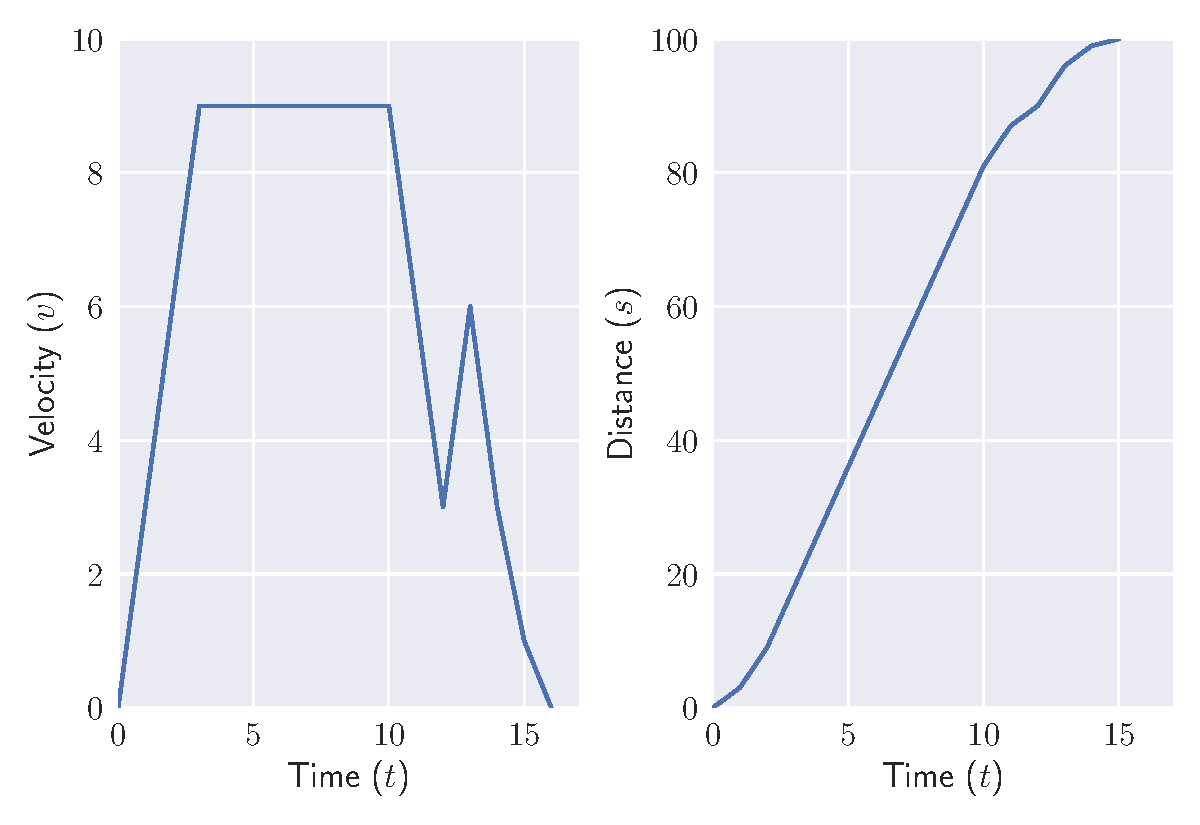
\includegraphics[scale=0.65]{fig/motor_control_graph.pdf}}
  % \vspace{-13mm}
\caption{Velocity ($v$) and distance travelled ($s$) plotted against time\label{fig-motor}}
\Description[Please consult the text of this section for the description]{}
\end{figure}

To be deployed into REDFIN, the algorithm~\ref{alg-motor} must be manually
re-implemented in REDFIN assembly. The resulting assembly program comprises 85 lines of
assembly and closely mirrors the high-level pseudocode. As a sample, consider a fragment of
the program's symbolic execution tree that corresponds to the decision whether to
accelerate, keep speed or decelerate the motor~\ref{fig-sym-tree}.

\begin{figure}[h]
\centerline{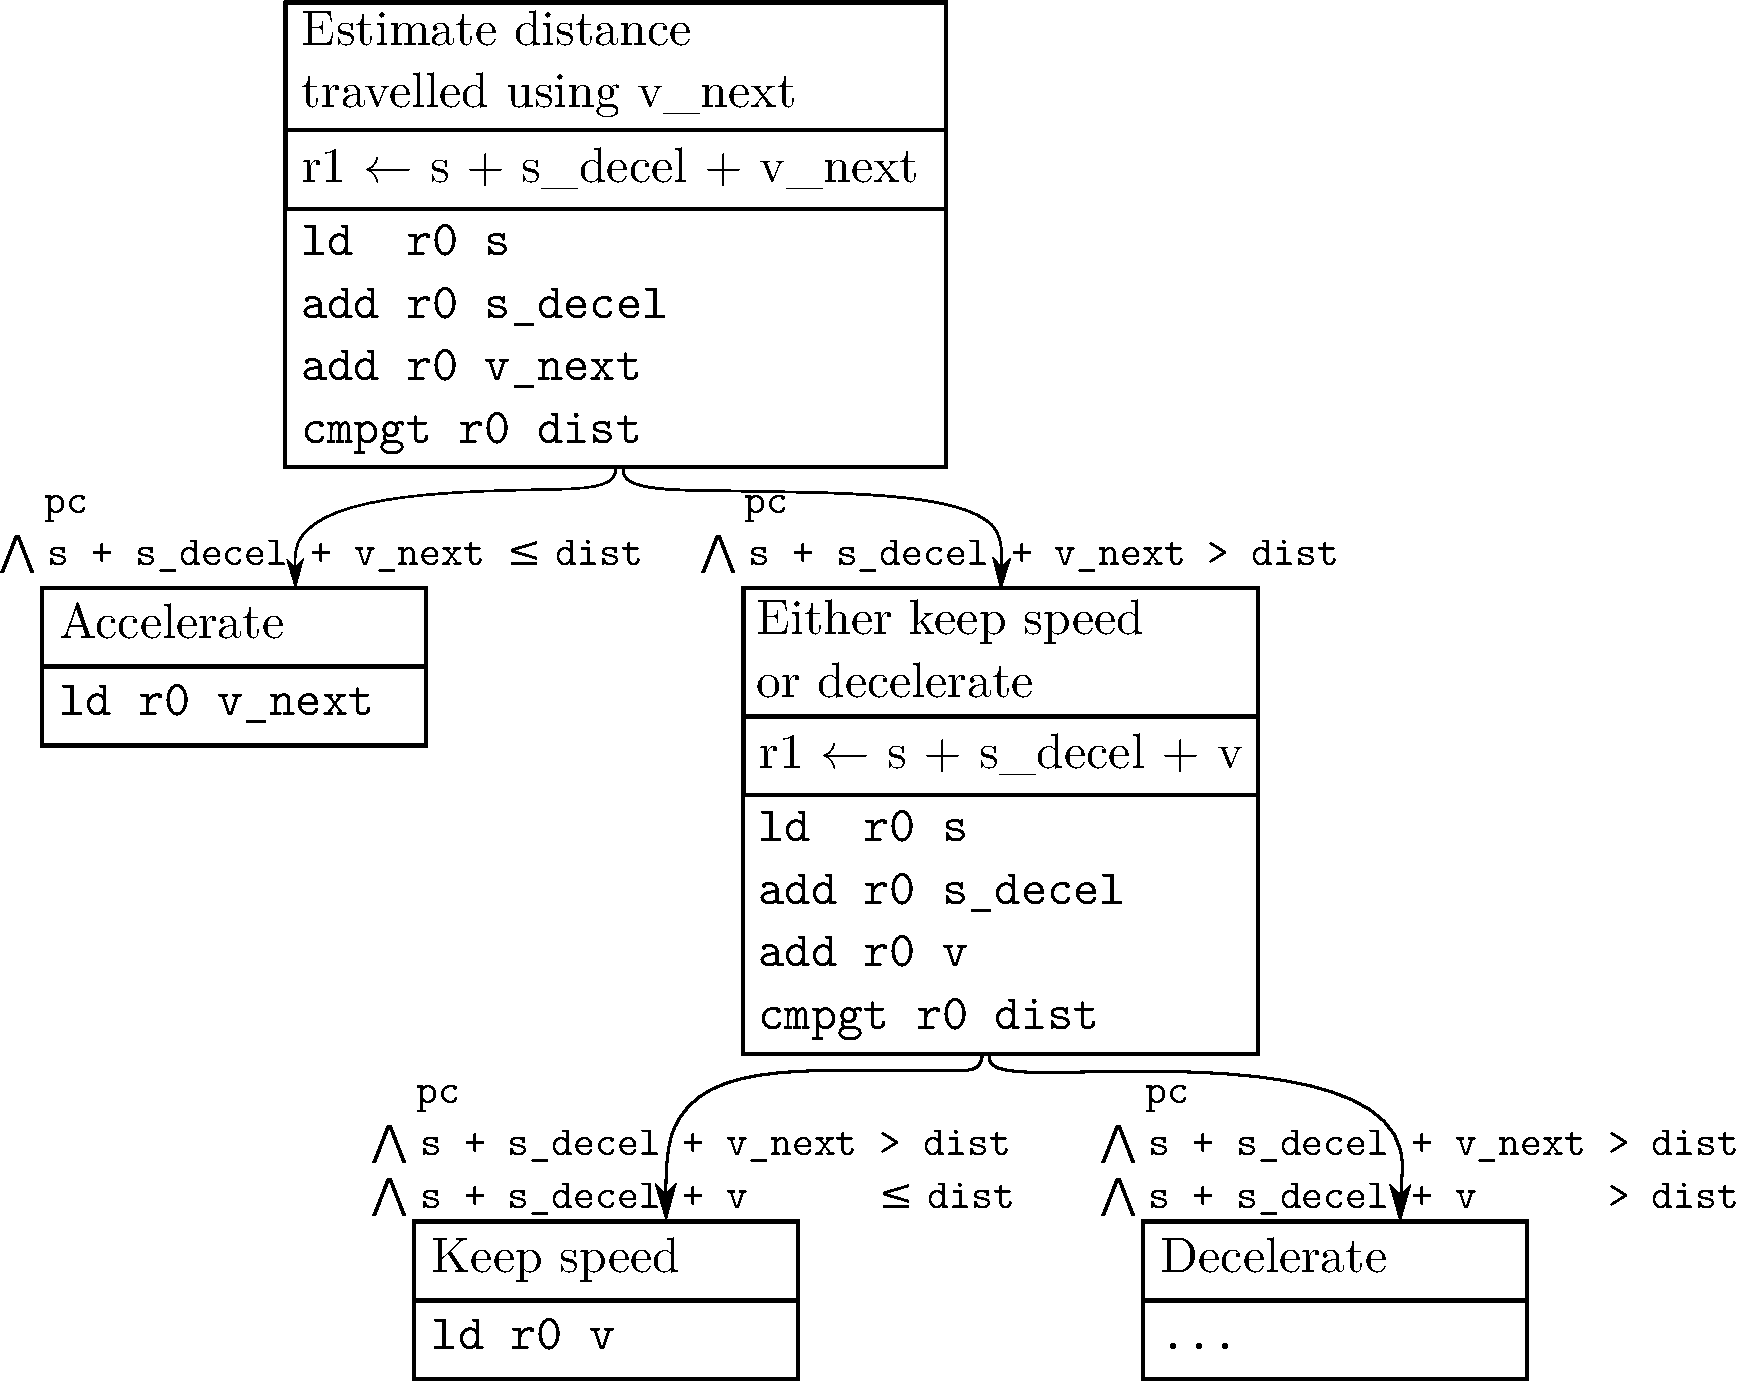
\includegraphics[scale=0.4]{fig/sym-tree-1.pdf}}
\caption{Symbolic execution tree of code fragment with conditional branching\label{fig-sym-tree}}
\Description[Please consult the text of this section for the description]{}
\end{figure}

The decision is based on first estimating the resulting distance travelled using
the next potential value $v\_next$ as velocity and if $dist$ is not covered by that
the motor will be accelerated; otherwise the resulting distance gets estimated
using the current velocity $v$ and in case $v$ is sufficient it is kept as the
velocity; otherwise the motor will be decelerated. The changes of speed may be
also seen from the velocity against time plot~\ref{fig-motor}.


\subsection{Loop invariant verification}

In order to ensure that the motor will not introduce disturbances
and will not lead the whole unit out of its normal mode of operation, the velocity and
acceleration of the motor must be kept in safe limits. This verification condition
is motivated by the correctness requirements of the whole space satellite unit.

More formally, the verification condition means
that in any iteration of the control program loop the values of the
expressions $v$, the velocity, and $\left| v\_next - v \right|$,
the acceleration, must never exceed the parameters $v\_max$ and $a\_max$, respectively.
This property is the loop invariant for the motor control program which
ensures that velocity and acceleration always stay within their safe bounds. We
formalise it as the following predicate that universally quantifies over the
program's inputs and the loop's state:

\begin{tcolorbox}
\LARGE{
\[
  \forall\ v\_max\ a\_max\ v\ v\_next\ s,
  \ v \leq v\_max \land \left| v\_next - v \right| \leq a\_max
\]}
\end{tcolorbox}

\noindent
We will verify the loop invariant by using the verification framework in the
\emph{branching mode}\ref{sec-operation-modes}. While symbolic execution with
merging, which is implemented by the framework's \emph{mergin} mode, allows
for intuitive formulation of properties for whole-program verification and
is very useful for verifying finite programs, as we have
reported in the section~\ref{sec-verification}, in presence of branches guarded
by symbolic values, it suffers from \emph{symbolic non-termination}.
Thus, for verifying the loop invariant, we rely on traditional symbolic execution.

To verify the loop invariant we take the following approach:

\begin{itemize}
  \item Obtain the binary tree-shaped trace by \emph{bounded} symbolic execution
  in \emph{branching} mode
  \item Split the trace into linear paths, thus enumerating all the possible
    execution scenarios
  \item For every path perform the analysis
    \begin{enumerate}
      \item Extract the relevant parts of the state from the \emph{last} node in
            the path, i.e. symbolic expressions stored in
            registers, memory cells or flags
      \item Construct a symbolic expression representing the \emph{property to check},
            which would involve the expressions obtained in the previous step
      \item Extract the \emph{path condition} from the /last/ node in the path
      \item Formulate the \emph{preconditions} of the program
      \item To verify the property in the given path by checking the following
            formula for satisfiability:
              preconditions /\ path constraints /\ ¬ property to check
    \end{enumerate}
    \item  The property holds if and only if for every path the solver returns
           \hs{Unsatisfiable}, i.e. there are no assignments of the variables which
           satisfy the~\emph{negation} of the property to check, considering the
           preconditions and the path condition.
\end{itemize}

This detailed verification algorithms has several parameters that need to be specified:

\begin{itemize}
\item Preconditions on $v\_max$ and $a\_max$
\item Symbolic execution bound, i.e. for how many steps perform the execution. Since the
      body of the loop will always terminate this bound can be calculated in advance.
\end{itemize}

\subsection{Pruning branches}

As illustrated by figure~\ref{fig-sym-tree}, every conditional jump instruction produces
two branches in the symbolic execution tree: the one
where the current path condition is conjoined with the jump's guard and the one where it is
conjoined with the guard's negation. However, if the resulting
conjunction is unsatisfiable, the corresponding branch does not have to be explored
and can be pruned. Thus the symbolic execution engine need to call an SMT solver every
time a conditional jump is encountered to check if the path conditions of the branches
are satisfiable.

Checking satisfiability of execution path is essential to mitigation the path explosion
problem. Pre-condition, when available, is assigned as the initial path condition and thus
will become a subterm of every formula submitted to the solver. Identifying correct preconditions
is essential for verification since they may drastically reduce the number of satisfiable paths
in the symbolic execution tree of the program that is being verified.


Give the preconditions, an example of the execution path, talk about constant folding
and SMT-solving to prove unsatisfiable paths, make a table(?) with results for different
preconditions: number of path, time to solve a path, length of the path maybe.

\subsection{NOTES}

``Pre-conditions, when
available, may be leveraged to reduce the size of the input
data domains and to only generate test inputs that satisfy
the pre-conditions.''


---
